\section{Scene}

Collinear points in the 3D space are projected onto collinear points in the image plane, preserving collinearity. 
This is achieved through a linear mapping between homogeneous coordinates.

The backprojection of an image point $\mathbf{u}$ for a camera $\mathbf{P}=\begin{bmatrix} \mathbf{M} & \mathbf{m} \end{bmatrix}$ traces a straight line through the origin $\mathbf{O}=\text{RNS}(\mathbf{P})$. 
The direction of this line is determined by $\mathbf{d}=\mathbf{M}^{-1}\mathbf{u}$.
\begin{figure}[H]
    \centering
    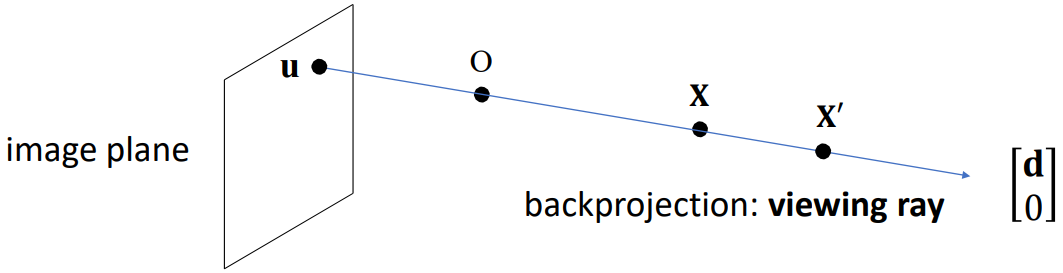
\includegraphics[width=0.4\linewidth]{images/scene.png}
    \caption{Scene}
\end{figure}